\chapter{Analisis}
\label{chap:analisi}

Pada bab ini akan dibahas mengenai analisis aplikasi sejenis, analisis kebutuhan aplikasi, analisi kontrol yang dipakai, analisis terhadap siklus hidup aplikasi, analisis peta, analisis pemanfaatan sumber data, analisis Kiri API, diagram \textit{Use Case}, dan diagram kelas.

%Analisis Aplikasi Sejenis
\section{Analisis Aplikasi Sejenis}
\label{lab:Analisis Aplikasi Sejenis}
% Aplikasi publik transport Android
\hspace{0.5cm} Aplikasi sejenis yang penulis temui bernama Public Transport\footnotemark[1]. Namun aplikasi Public Transport tersebut hanya dapat dijalankan di sistem aplikasi android. Aplikasi Public Transport ini memanfaatkan Kiri API. Aplikasi tersebut penggunaannya sederhana. Di halaman awal pengguna dapat mengetikan lokasi awal dan tujuan. Selain dengan mengetik pengguna juga dapat menunjuk lokasi pada peta. Setelah lokasi dipilih sistem akan memastikan dengan memberi daftar nama jalan dan tempat terkait. Jika sudah memilih maka sistem akan mengeluarkan hasil pencarian rute.
\footnotetext[1]{\url{https://play.google.com/store/apps/details?id=travel.kiri.smarttransportapp}}

Berikut adalah tampilan dari aplikasi Public Transport (Gambar ~\ref{fig:home} sampai ~\ref{fig:peta}):

\begin{figure}[h]
	\centering
		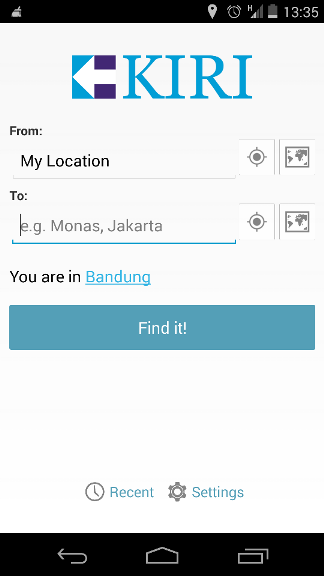
\includegraphics[scale=0.5]{Gambar/KIRI_Android/home}
	\caption{Tampilan utama aplikasi Public Transport}
	\label{fig:home}
\end{figure}

Gambar ~\ref{fig:home} menunjukan halaman utama aplikasi Public Transport. Di halaman ini pengguna dapat memasukan lokasi asal dan lokasi tujuan. Cara memasukan lokasi ada 2 macam yaitu dengan mengetik dan menunjuk pada peta dengan mengetuk tombol peta. Bila pengguna ingin menunjuk lokasi pengguna berada dapat dilakukan dengan mengetuk tombol kordinat. Tersedia juga pelihan kota yang dapat dipilih oleh pengguna.

\begin{figure}[h]
	\centering
		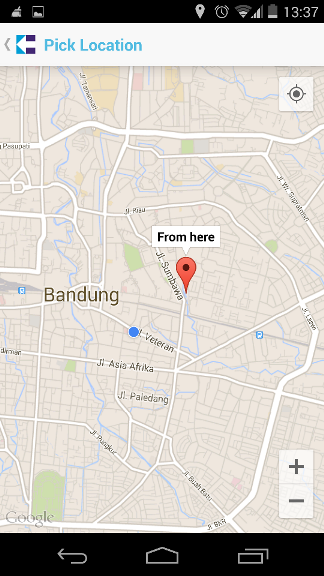
\includegraphics[scale=0.5]{Gambar/KIRI_Android/menunjuk_lokasi}
	\caption{Menunjuk lokasi pada peta}
	\label{fig:menunjuk}
\end{figure}

Gambar ~\ref{fig:menunjuk} jika pengguna sudah mengetahui lokasi namun tidak tahu nama lokasi. Pada halaman ini pengguna diarahkan untuk menemukan lokasi pada peta dan mengetuk lokasi tersebut untuk memilihnya.

\begin{figure}[h]
	\centering
		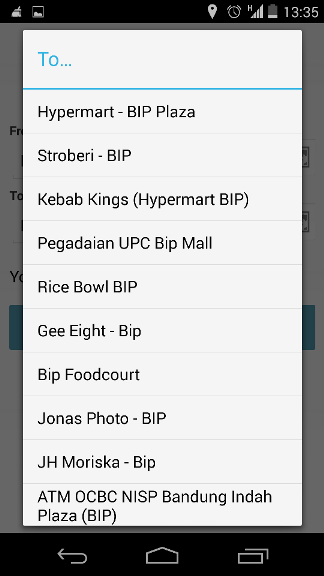
\includegraphics[scale=0.5]{Gambar/KIRI_Android/terkait}
	\caption{Memberikan daftar nama tempat dan nama jalan terkait}
	\label{fig:terkait}
\end{figure}

Pada gambar ~\ref{fig:terkait} pengguna dapat memilih nama tempat terkait. Pemilihan didasarkan sesuai masukan pengguna untuk memastikan tempat asal maupun tempat tujuan. Jika nama tempat sudah jelas maka tidak akan ada halaman ini.

\begin{figure}[h]
	\centering
		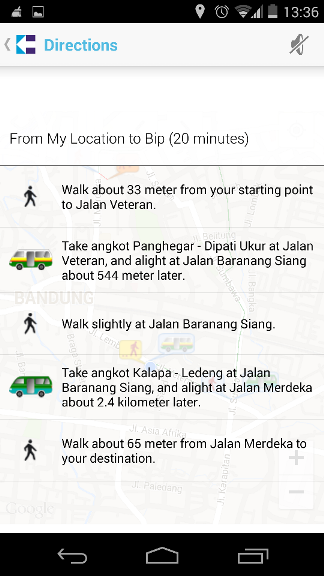
\includegraphics[scale=0.5]{Gambar/KIRI_Android/tampilan_daftar}
	\caption{Tampilan rute kendaraan umum dalam bentuk daftar}
	\label{fig:daftar}
\end{figure}

Pada gambar ~\ref{fig:daftar} menampilkan daftar rute kendaraan umum yang harus dinaiki beserta gambar untuk mempermudah pengguna. Selain itu disertakan juga jarak dan perkiraan waktu sampai di lokasi tujuan.

\begin{figure}[h]
	\centering
		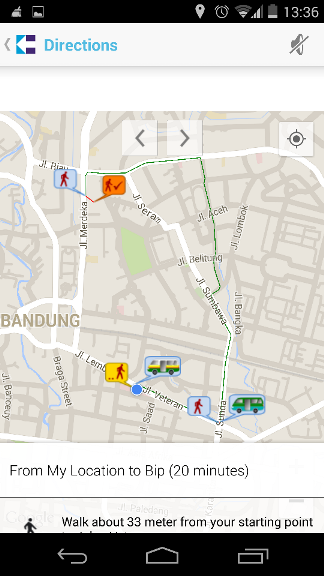
\includegraphics[scale=0.5]{Gambar/KIRI_Android/tampilan_peta}
	\caption{Tampilan rute kendaraan umum di peta}
	\label{fig:peta}
\end{figure}

Pada gambar ~\ref{fig:peta} menampilkan rute kendaraan umum dan jalur yang harus dilalui pada peta. Dengan cara ini pengguna dapat mengetahui posisi dan jalur yang harus dilalui.

% tampilannya, cara kerja, hal yang dapat dilakukan

\clearpage

%Analisis Analisis Program
\section{Analisis Aplikasi}
\label{lab:Analisis Aplikasi}
\hspace{0.5cm} Aplikasi akan dibuat menggunakan bahasa pemograman C\#. Aplikasi yang digunakan untuk membangun Aplikasi Pencari Rute Kendaraan Umum untuk Windows Phone adalah Visual Studio Express 2012. Pada sub bab ini akan dibahas kebutuhan aplikasi, anaslisis kontrol yang dipakai, analisis terhadap siklus hidup aplikasi, analisis peta, analisis pemanfaatan sumber data, analisa Kiri API, diagram \textit{use case}, dan diagram kelas dari aplikasi yang akan dibangun. 

%Analisis Kebutuhan Aplikasi
\subsection{Kebutuhan Aplikasi}
\label{lab:Kebutuhan Aplikasi}
\hspace{0.5cm} Dari hasil observasi penulis dalam menentukan lokasi asal dan lokasi tujuan ada dua cara. Kedua cara tersebut yaitu dengan menulis alamat atau tempat dan dengan menunjuk pada peta. Cara menuliskan alamat atau tempat yaitu dengan menuliskan alamat atau tempat pada tempat yang disediakan untuk asal dan tujuan. Cara menunjuk pada peta yaitu dengan mengetuk layar di posisi yang diinginkan. Kedua hal tersebut pada dasarnya sama saja tetapi ada faktor kemudahan pengguna dalam pemakaiannya. Jadi penulis menyediakan dua cara tersebut pada aplikasi yang penulis buat agar pengguna dapat memilih salah satunya.

Pada saat menuliskan lokasi atau tempat atau menunjuk langsung pada peta mungkin saja terjadi kesalahan. Kesalahan tersebut bisa saja disebabkan salah pengetikan atau nama tempat yang tidak ada. Maka dari itu dibutuhkan pemeriksaan terhadap masukan pengguna. Pemeriksaan tersebut dilakukan setelah pengguna memulai pencarian dengan menekan tombol "FIND".

Untuk hasil keluaran ada dua tipe seperti aplikasi peta lainnya. Kedua tipe tersebut adalah bentuk daftar dan bentuk peta. Bentuk daftar memudahkan dalam melihat tiap langkah rute. bentuk daftar memudahkan pengguna dalam melihat arah dan posisi lingkungan pada rute yang dipilih.

\hspace{0.5cm} Aplikasi yang penulis bangun didasarkan pada kebutuhan sebagai berikut.
\begin{enumerate}
	\item Pengguna dapat memasukan lokasi asal dan lokasi tujuan pada \textit{TextBox} yang disediakan atau menunjuk langsung lokasi pada peta.
	\item Mendapatkan lokasi terkait menurut lokasi yang dimasukan pengguna.
	\item Menampilkan hasil rute angkutan umum dari lokasi asal ke lokasi tujuan.
\end{enumerate}

% SUB Analisis Kontrol yang Dipakai
\subsection{Analisis Kontrol yang Dipakai}
\label{lab:Analisis Kontrol yang Dipakai}
\hspace{0.5cm} Dari kebutuhan yang telah disebutkan diatas penulis menyadari pentingnya kontrol yang harus dipakai. Kontrol yang dimaksud termasuk tata letak, teks, pilihan, dan daftar. Kebutuhan akan kontrol penting bukan hanya untuk kebutuhan tapi memudahkan pengguna.

Untuk kontrol tata letak penulis membayangkan pengaturan yang tertata rapih dan beberapa elemen dalam satu baris atau kolom. Tetapi juga penulis tidak mengharapkan penggunaan kontrol tata letak yang rumit. Dari hasil pengamatan penulis kontrol tata letak yang cocok adalah Grid. Kontrol tata letak ini penulis pilih karena mudah diposisiskan sesuai baris dan kolom. Selain itu tampilan Grid akan menyesuaikan jika layar diputar dari posisi pemandangan ke posisi potret dan sebaliknya.

Kontrol terhadap teks juga diperlukan untuk aplikasi. Kebutuhan yang diperlukan adalah mengeluarkan potongan teks yang dapat dibaca dan tempat pengguna memasukan teks. Untuk mengeluarkan teks yang dapat dilihat penulis akan menggunakan \textit{TextBlock}. TextBlock digunakan untuk menampilkan tulisan "from" dan "to" pada halaman utama aplikasi. Untuk masukan pengguna terhadap aplikasi penulis akan menyediakan \textit{TextBox} sebagai tempat teks. \textit{TextBox} digunakan sebagai masukan untuk lokasi asal dan lokasi tujuan.

Suatu aplikasi tentunya tidak hanya mempunyai satu halaman. Sama hal dengan aplikasi yang penulis buat memiliki beberapa halaman yang mempunyai tugas berbeda. Karena hal tersebut dibutuhkan kontrol untuk berpindah dari satu halaman ke halaman lain. Kontrol yang dibutuhkan yaitu kontrol tombol. Kontrol tombol akan mengeksekusi \textit{event click} yang memungkinkan pindah halaman dan melakukan perintah. Kontrol tombol akan penulis gunakan untuk berpindah ke halaman peta, menemukan lokasi pengguna, dan pencarian rute. Pada Gambar~\ref{fig:antarmuka} terdapat 5 tombol yaitu tombol map pada bagian from, tombol here pada bagian from, tombol map pada bagian to, tombol here pada bagian to, dan tombol find. Berikut kegunaan dari tombol-tombol tersebut.
\begin{itemize}
	\item Tombol map pada bagian from\\
	Tombol untuk berpindah dari halaman utama menuju halaman peta. Pada halaman peta pengguna dapat menunjuk lokasi asal dan kembali lagi ke halaman utama. Saat kembali ke halaman utama lokasi yang dipilih akan disimpan dan pada \textit{TextBox} bagian from akan tertulis "lokasi dari peta".
	\item Tombol map pada bagian from\\
	Tombol untuk mancari lokasi pengguna. Setelah tombol ini di tekan maka lokasi pengguna akan disimpan dan pada bagian \textit{TextBox} bagian from akan tertulis "here".
	\item Tombol map pada bagian to\\
	Tombol untuk berpindah dari halaman utama menuju halaman peta. Pada halaman peta pengguna dapat menunjuk lokasi tujuan dan kembali lagi ke halaman utama. Saat kembali ke halaman utama lokasi yang dipilih akan disimpan dan pada \textit{TextBox} bagian to akan tertulis "lokasi dari peta".
	\item Tombol map pada bagian to\\
	Tombol untuk mancari lokasi pengguna. Setelah tombol ini di tekan maka lokasi pengguna akan disimpan dan pada bagian \textit{TextBox} bagian to akan tertulis "here".
	\item Tombol find 
	Tombol ini akam mencari rute angkutan umum dan menampilkannya pada halaman peta.
\end{itemize}

Pada aplikasi ini penulis akan menampilkan daftar tempat dan daftar rute angkutan umum yang dipakai. Bentuk daftar digunakan penulis karena hasil tempat dan rute angkutan umum akan banyak. Bentuk daftar yang dapat dipakai di Windows Phone adalah menggunakan \textit{ListBox}. \textit{ListBox} akan menampilkan daftar tempat dan daftar rute satu per satu menurun ke bawah.

% SUB Analisis Terhadap Siklus Hidup Aplikasi
\subsection{Analisis Terhadap Siklus Hidup Aplikasi}
\label{lab:Analisis Terhadap Siklus Hidup Aplikasi}
\hspace{0.5cm} Aplikasi pada Windows Phone memiliki siklus hidup yang dijelaskan pada bab ~\ref{subsec:Siklus Hidup Aplikasi}. Pengaturan aplikasi ini diatur sesuai konfigurasi awal sistem operasi Windows Phone. Tetapi pengaturan ini dapat diatur sesuai kebutuhan aplikasi. Karena di aplikasi ini terdapat keadaan yang berbeda dengan konfigurasi awal sistem operasi Windows Phone maka perlu dilakukan pengaturan ulang siklus hidup.

Saat aplikasi dijalankan, pengguna memasukan lokasi asal dan lokasi tujuan. Setelah memasukan lokasi pengguna akan mencari rute. Ketika rute berhasil ditemukan aplikasi akan berada di keadaan Running. Tetapi ada kemungkinan pengguna berpindah aplikasi atau mematikan layar untuk menghemat daya. Dalam kasus tersebut sistem operasi Windows Phone akan menganggap aplikasi tidak aktif dan aplikasi akan masuk pada keadaan \textit{dormant}. Untuk menangani kasus tersebut maka penulis harus menyimpan keadaan dan informasi saat sebelum aplikasi menjadi tidak aktif. Penanganan yang penulis akan lakukan adalah menggunakan metode \textit{OnNavigatedFrom()}. Dengan metode tersebut keadaan aplikasi akan disimpan di memori.

Pada saat aplikasi masuk keadaan Dormant semua \textit{thread} dan proses akan dihentikan. Pada saat tersebut juga GPS Windows Phone akan terhenti dan tidak akan mengetahui posisi pengguna. GPS akan kembali aktif mengetahui posisi pengguna jika pengguna masuk ke aplikasi dan tentunya membutuhkan waktu untuk pelacakan lokasi. Tetapi Windows Phone mendukung proses di belakang untuk pelacakan GPS selama keluar dari aplikasi atau layar perangkat dimatikan. Maka dari itu aplikasi yang penulis buat akan mendukung pengaksesan lokasi meskipun layar perangkat dimatikan atau berpindah aplikasi. 

Ketika aplikasi sudah berada pada keadaan \textit{Dormant} atau \textit{Tombstoned}, pengguna masih dapat memulihkan keadaan aplikasi saat aplikasi berada di keadaan \textit{Running} sebelumnya. Penanganan yang penulis akan lakukan untuk hal tersebut adalah menggunakan metode \textit{OnNavigatedTo()}. Menggunakan metode tersebut akan memulihkan informasi halaman pada keadaan \textit{Running} sebelumnya.
%mendukung backgorund execution, running bacground event

% SUB Analisis Peta
\subsection{Analisis Peta}
\label{lab:Analisis Peta}
\hspace{0.5cm} Untuk tampilan peta ada beberapa aspek yang perlu diperhatikan untuk memudahkan pengguna. Aspek yang perlu diperhatikan adalah sebagai berikut.
\begin{itemize}
	\item Pemetaan terhadap peta atau \textit{cartographic} dan mode warna
	\item Tingkat \textit{zoom}
	\item Menampilkan gambar dan keterangan angkutan umum menggunakan \textit{pushpin}
	\item Menggambar rute pada peta menggunakan \textit{polyline}
\end{itemize}

Untuk cara pandang peta terdapat 4 pandangan yang disediakan peta di Windows Phone yaitu \textit{Road}, \textit{Aerial}, \textit{Hybrid}, dan \textit{Terrain}. Aplikasi ini adalah aplikasi pencari rute dan pandangan lebih banyak diarahkan ke jalanan perkotaan. Kebutuhan pengguna adalah nama jalan, kondisi jalan, dan kondisi sekitar. Dari dasar pandangan tersebut pandangan yang penulis pilih untuk aplikasi ini adalah \textit{Road}. Tambahan setelah mengatur pandangan peta yaitu mengatur warna dan penulis akan menggunakan mode warna terang sesuai bawaan peta di Windows Phone.

Tampilan awal peta di Windows Phone akan mengeluarkan peta dengan pandangan dunia. Karena aplikasi pencarian rute ini masih terbatas di Pulau Jawa, Indonesia terutama Jawa Barat maka tingkat zoom harus diatur agar mengikuti lokasi pengguna dan di satu daerah saja. Jika pengguna berada di daerah Bandung maka tingkat zoom pada peta disesuaikan pada daerah tersebut. Tingkat zoom dapat dapat diatur dari kode dan XAML. Tingkat zoom yang penulis akan gunakan adalah 14. Tingkat zoom 14 akan menampilkan satu kota dengan jelas.
%kasih gambar zoom 14

Di setiap kota ada satu angkutan umum yang banyak dipakai yaitu angkutan kota(angkot). Namun bagi yang baru pertama mengunjungi suatu daerah dan mencari angkot mungkin akan kesulitan membaca trayek dari angkot tersebut. Namun ada satu cara yang mudah untuk membedakan angkot di setiap rute yaitu dari warna dan coraknya. Agar dapat memudahkan pengguna dan menghindari pengguna dari kesalahan naik angkot maka Kiri API sudah menyediakan gambar angkot yang seusai dengan setiap rute. Gambar angkot tersebut akan ditempatkan di peta dengan suatu penampung beserta keterangannya. Salah satu teknik untuk menempatkan gambar tersebut adalah dengan membuat lapisan terpisah di atas peta tempat gambar tersebut. Untuk hal tersebut penulis akan memanfaatkan Pushpin sebagai lapisan terpisah untuk menaruh gambar dan keterangan angkutan umum. Berikut tampilan \textit{pushpin} untuk angkot~\ref{fig:pushpin_angkot} dan \textit{pushpin} untuk jalan kaki~\ref{fig:pushpin_jalan}.

\begin{figure}[h]
	\centering
		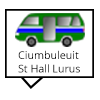
\includegraphics[scale=0.5]{Gambar/out_kiri/angkot}
	\caption{Tampilan \textit{pushpin} untuk angkot}
	\label{fig:pushpin_angkot}
\end{figure}

\begin{figure}[h]
	\centering
		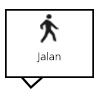
\includegraphics[scale=0.5]{Gambar/out_kiri/jalan}
	\caption{Tampilan \textit{pushpin} untuk jalan kaki}
	\label{fig:pushpin_jalan}
\end{figure}

Pencarian rute yang penulis gunakan untuk aplikasi yaitu dengan memakai Kiri API. Kiri API akan memberikan kembalian berupa titik-titik rute perjalanan dari lokasi asal ke lokasi tujuan. Karena hal itu penulis harus menggambar rute tersebut sesuai jalan pada peta. Untuk hal tersebut penulis akan menggunakan \textit{Polyline} pada Windows Phone untuk menggambarnya. \textit{Polyline} yang digambar harus terlihat dengan jelas dan diberi warna yang kontras dengan tampilan peta. Warna polyline yang penulis akan pilih adalah merah dengan ketebalan 2.

% SUB Analisis Pemanfaatan Sumber Data
\subsection{Analisis Pemanfaatan Sumber Data}
\label{lab:Analisis Pemanfaatan Sumber Data}
\hspace{0.5cm} Aplikasi yang penulis buat memanfaatkan sumber data dari luar. Sumber data yang penulis dapatkan dalam format JSON (\textit{Javascript object Notation}). Pengambilan sumber data tersebut dilakukan dengan melakukan permintaan HTTP dari \textit{Uniform Resource Identifier} / URI. Pemanfaatan sumber data yang penulis gunakan adalah kelas \textit{HttpClient}.

Metode yang penulis gunakan adalah \textit{GetStringAsync()}. Metode ini akan mengirimkan permintaan melalui URI dan mengembalikan hasilnya dalam tipe data \textit{String} dan kemajuan data. Karena metode ini mengembalikan hasil dalam tipe data \textit{String} maka mudah disesuaikan dengan kebutuhan tugas akhir ini. Selanjutnya penulis harus membuat pengurai untuk keluaran  untuk diolah menjadi informasi yang dibutuhkan.   
%penggunaan getString

% SUB Analisis Kiri API
\subsection{Analisis Kiri API}
\label{lab:Analisis Kiri API}
%parameter get karena hanya untuk mendapatkan data dan tidak ada data sensiti yg dikirimkan.
\hspace{0.5cm} Kiri API menyediakan 2 parameter untuk permintaan yaitu \textit{POST} dan \textit{GET}. Dalam tugas akhir ini penulis akan menggunakan parameter \textit{GET}. Parameter \textbf{GET} penulis pilih karena dalam tugas akhir ini penulis akan banyak mendapatkan data dan tidak ada data sensitif yang dikirimkan. Untuk hal ini penulis akan mengirim ke URL \url{http://kiri.travel/handle.php}.

Untuk setiap permintaan terhadap Kiri API dibutuhkan \textit{API key}. Kegunaan \textit{API key} adalah password untuk mengakses Kiri API. \textit{API key} dapat didapatkan di \url{dev.kiri.travel}. \textit{API key} yang penulis gunakan pada tugas akhir ini adalah 97A7A1157A05ED6F.
     
Untuk tugas akhir ini penulis akan menggunakan 2 layanan yang ada pada Kiri API. Layanan yang digunakan adalah pencarian lokasi dan penentuan rute. Pencarian lokasi adalah layanan untuk menemukan tempat atau nama jalan yang terkait dengan masukan pengguna. Penentuan rute adalah layanan untuk menemukan langkah yang harus ditempuh pengguna untuk sampai ke lokasi tujuan dari lokasi asal. 

Pemanfaatan layanan pencarian lokasi yaitu dengan parameter \textit{GET} melalui protokol HTTP. Berikut parameter yang harus dikirimkan beserta keterangannya.
\begin{itemize}
	\item \textit{version}: 2 \\
	Karena acuan penulis adalah Kiri API versi maka di parameter version penulis akan menggunakan 2.
	\item \textit{mode}: "searchplace" \\
	Mode "searchplace" digunakan untuk mencari lokasi terkait.
	\item \textit{region}: "cgk" untuk Jakarta, "bdo" untuk Bandung, dan "sub" untuk Surabaya \\
	Karena Kiri API baru tersedia di 3 kota yaitu Jakarta, Bandung, dan Surabaya maka region harus dimasukan untuk pencarian. Region harus dipilih antara "cgk"/"bdo"/"sub" sebagai parameter. Pengguna dapat menentukan masukan region jika menuliskannya pada lokasi asal atau lokasi tujuan. Tetapi, jika pengguna tidak menuliskannya maka sistem yang akan menentukan. Cara penentuan region oleh sistem adalah sistem akan menampung titik tengah dari ketiga region tersebut lalu membandingkannya dengan lokasi pengguna berada. Jarak terdekat antara lokasi pengguna dan salah satu region menandakan pengguna berada di region tersebut.
	\item \textit{querystring}: merupakan kata kunci lokasi 
	\item \textit{apikey}: 16 digit heksadesimal
\end{itemize}
Format layanan yang dikirim melalui URL adalah \url{kiri.travel/handle.php?version=2&mode=searchplace&region=cgk/bdo/sub&querystring="string"&apikey=97A7A1157A05ED6F}.
\newline
\\Penulis mencoba mencari lokasi bip dari kata kunci "bip" yang berada di bandung. Layanan dikirimkan ke URL \url{kiri.travel/handle.php}. 
Berikut format layanan yang penulis kirim:\newline
{\url{http://kiri.travel/handle.php?version=2&mode=searchplace&region=bdo&querystring=bip&apikey=97A7A1157A05ED6F}}
\newline
\\Berikut hasil kembalian dari Kiri API: 

\begin{lstlisting} [caption= Kode kembalian dari pencarian rute]
{ 
	"status":"ok",
	"searchresult":[
		{
			"placename":"Hypermart - BIP Plaza",
			"location":"-6.90864,107.61108"
		},
		{
			"placename":"Stroberi - BIP",
			"location":"-6.90834,107.61115"
		},
		{
			"placename":"Kebab Kings (Hypermart BIP)",
			"location":"-6.91503,107.61017"
		},
		{
			"placename":"Pegadaian UPC Bip Mall",
			"location":"-6.90916,107.61052"
		},
		{
			"placename":"Rice Bowl BIP",
			"location":"-6.90873,107.61088"
		},
		{	
			"placename":"Gee Eight - Bip",
			"location":"-6.90817,107.61080"
		},
		{
			"placename":"Jonas Photo - BIP",
			"location":"-6.91066,107.61016"
		},
		{
			"placename":"Bip Foodcourt",
			"location":"-6.91081,107.61015"
		},
		{
			"placename":"Mister Baso BIP",
			"location":"-6.90348,107.61709"
		},
		{
			"placename":"JH Moriska - Bip",
			"location":"-6.90868,107.61070"
		}
	],
	"attributions":null
}
\end{lstlisting}

Hasil dari kembalian berupa kumpulan \textit{placename} dan \textit{location}. Hasil tersebut akan aplikasi tampung namun yang akan ditampilkan ke pengguna hanya \textit{placename}. Menampilkan \textit{location} tidak efektif menurut penulis karena akan membingungkan pengguna. Dari percobaan yang penulis lakukan, nilai dari \textit{attributions} selalu bernilai "null". Karena hal tersebut maka nilai\textit{attributions} akan penulis abaikan.

Pemanfaatan layanan penentuan rute untuk mendapatkan langkah yang harus ditempuh pengguna untuk mencapai lokasi tujuan dari lokasi asal. Pemanfaatan layanan ini yaitu dengan parameter \textit{GET} melalui protokol HTTP. Berikut parameter yang harus dikirim:
\begin{itemize}
	\item \textit{version}: 2 \\
	Karena acuan penulis adalah Kiri API versi maka di parameter version penulis akan menggunakan 2.
	\item \textit{mode}: "findroute" \\
	Mode "findroute" digunakan untuk mendapatkan langkah yang harus ditempuh menuju lokasi tujuan.
	\item \textit{locale}: "en" untuk bahasa Inggris dan "id" untuk bahasa Indonesia. \\
	Karena aplikasi ini memungkinkan dipakai orang banyak maka penulis putuskan untuk menggunakan bahasa Inggris.
	\item \textit{start}: koordinat lokasi awal dalam berupa latitude dan longitude. \\
	Masukan untuk lokasi awal harus dalam bentuk koordinat. Jika masukan dari pengguna adalah alamat atau tempat maka perlu dicari kordinatnya dahulu.
	\item \textit{finish}: koordinat lokasi tujuan dalam berupa latitude dan longitude. \\
	Masukan untuk lokasi tujuan harus dalam bentuk koordinat. Jika masukan dari pengguna adalah alamat atau tempat maka perlu dicari kordinatnya dahulu.
	\item \textit{presentation}: "mobile" untuk perangkat bergerak dan "desktop" untuk komputer. \\
	Karena aplikasi ini dirancang untuk Windows Phone 8, presentasi yang penulis pilih adalah "mobile".
	\item \textit{apikey}: 16 digit heksadesimal.
\end{itemize}

Format layanan yang dikirim melalui URL adalah \url{kiri.travel/handle.php?version=2&mode=findroute&locale=en/id&start=lat,lng&finish=lat,lng&presentation=mobile/desktop&apikey=97A7A1157A05ED6}

Penulis mencoba menuju jalan merdeka dari jalan ciumbuleuit. Layanan dikirimkan ke URL \url{kiri.travel/handle.php}. Berikut format layanan yang penulis kirim \url{http://kiri.travel/handle.php?version=2&mode=findroute&locale=en&start=-6.8747337,107.6048829&finish=-6.9114646,107.6104887&presentation=mobile&apikey=97A7A1157A05ED6F}.\\
\newline
Berikut hasil kembalian dari Kiri API:
\begin{lstlisting} [caption= Kode kembalian pencarian rute]
{
	"status":"ok",
	"routingresults":[
		{
			"steps":[
				[
					"walk",
					"walk",
					["-6.8747337,107.6048829","-6.87445,107.60465"],
					"Walk about 41 meter from your starting point \%fromicon to Jalan Ciumbuleuit \%toicon.",
					null
				],
				[
					"angkot",
					"ciumbuleuitsthalllurus",
					["-6.87445,107.60465","-6.87541,107.60443","-6.87637,107.60421","-6.87734,107.60400",
					"-6.87830,107.60378", "-6.87926,107.60356","-6.87926,107.60356","-6.87963,107.60352",
					"-6.87978,107.60352","-6.88093,107.60392","-6.88209,107.60433","-6.88209,107.60433",
					"-6.88328,107.60490","-6.88328,107.60490","-6.88347,107.60481","-6.88452,107.60459",
					"-6.88556,107.60436","-6.88660,107.60413","-6.88764,107.60390","-6.88764,107.60391",
					"-6.88782,107.60392","-6.88887,107.60404","-6.88991,107.60416","-6.88991,107.60416",
					"-6.89161,107.60428","-6.89161,107.60428","-6.89166,107.60421","-6.89275,107.60424",
					"-6.89275,107.60424","-6.89405,107.60408","-6.89405,107.60408","-6.89496,107.60400"],
					"Take angkot Ciumbuleuit - St. Hall (lurus) at Jalan Ciumbuleuit \%fromicon, and alight at Jalan Cihampelas 
					\%toicon about 2.3 kilometer later.",
					null
				],
				[
					"angkot",
					"kalapaledeng",
					["-6.89501,107.60403","-6.89562,107.60398","-6.89623,107.60395","-6.89732,107.60401",
					"-6.89732,107.60401","-6.89882,107.60414","-6.89882,107.60414","-6.89969,107.60418",
					"-6.90071,107.60426","-6.90173,107.60433","-6.90173,107.60433","-6.90297,107.60437",
					"-6.90420,107.60440","-6.90420,107.60440","-6.90426,107.60456","-6.90422,107.60481",
					"-6.90399,107.60546","-6.90406,107.60617","-6.90454,107.60697","-6.90454,107.60697",
					"-6.90512,107.60745","-6.90618,107.60778","-6.90618,107.60778","-6.90643,107.60787",
					"-6.90651,107.60807","-6.90675,107.60914","-6.90675,107.60914","-6.90694,107.60939",
					"-6.90723,107.60939","-6.90891,107.60943","-6.90891,107.60943","-6.90909,107.60934",
					"-6.90914,107.60857","-6.90933,107.60846","-6.91021,107.60887","-6.91021,107.60887",
					"-6.91030,107.60897","-6.91028,107.60927","-6.90986,107.61040","-6.90986,107.61040"],
					"Take angkot Kalapa - Ledeng at Jalan Cihampelas \%fromicon, and alight at Jalan Aceh 
					\%toicon about 2.3 kilometer later.",
					null
				],
				[
					"walk",
					"walk",
					["-6.90986,107.61040","-6.9114646,107.6104887"],
					"Walk about 178 meter from Jalan Aceh \%fromicon to your destination \%toicon.",
					null
				]
				],
					"traveltime":"30 minutes"
				}
			]
}
\end{lstlisting}

Setiap langkah akan aplikasi tampung dalam elemen \textit{array}. Untuk keterangan dan jenis angkutan umum akan aplikasi tampilkan dalam bentuk \textit{pushpin} pada peta atau daftar. Sedangkan untuk titik-titik kordinat akan digambarkan pada peta. Dari analisa penulis setiap langkah menunjukan perpindahan angkutan umum yang dipakai, berpindah dari angkutan umum atau jalan, dan dari jalan untuk menaiki angkutan umum. Keterangan yang penulis akan tambahkan harus berada antara setiap \textit{steps} tersebut. Dari analisa penulis juga terdapat kata "\%fromicon" dan "\%toicon" yang tidak menunjukan sesuatu. Karena itu kedua kata tersebut akan penulis hilangkan agar tidak mengganggu pengguna. Penulis juga akan mengambil gambar angkutan kota dan gambar jalan yang sudah disediakan dari Kiri dengan memanfaatkan URL yang disediakan. 

%Analisis Diagram Use-Case dan Scenario
\subsection{Diagram \textit{Use Case} dan Scenario}
\label{lab:Diagram Use-Case dan Scenario}
\hspace{0.5cm} Diagram \textit{use case} adalah diagram yang menjelaskan interaksi sistem dengan lingkungan (contoh: pengguna). Berdasarkan analisa di atas maka pengguna dapat:
\begin{itemize}
	\item Mendapatkan lokasi pengguna berada.
	\item Memasukan lokasi asal dan lokasi tujuan.
	\item Menunjuk langsung lokasi asal dan tujuan pada peta.
	\item Memilih alamat atau tempat dari pilihan yang disediakan.
	\item Menampilkan rute kendaraan umum dalam bentuk titik dan \textit{pushpin} pada peta atau bentuk daftar dari tempat asal ke tempat tujuan.
\end{itemize}

\newpage
Diagram \textit{use case} saat pengguna mencari rute kendaraan umum dapat dilihat pada gambar (Gambar:~\ref{fig:UseCase}):
% Use case
\begin{figure}[h]
	\centering
		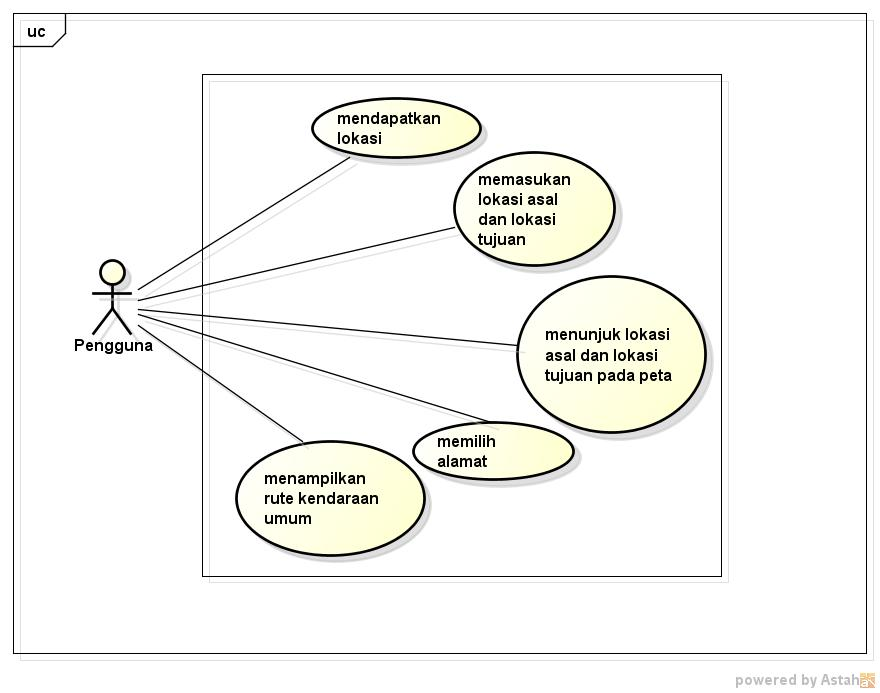
\includegraphics[scale=0.5]{Gambar/useCase_dan_Class/UseCase}
	\caption{Diagram \textit{use case}}
	\label{fig:UseCase}
\end{figure}

Skenario pencarian rute kendaraan umum dapat dilihat pada tabel~\ref{tab:mandapatLokasi} sampai tabel~\ref{tab:menampilkan}.
%\vtop{\hbox{\strut kalimat_1} \hbox{\strut kalimat_2}}
\begin{table}[H]
	\centering
		\begin{tabular}{ |p{2cm}|p{10cm}| }
			\hline
			Nama &  Mendapatkan lokasi perangkat\\ \hline
			Aktor & Pengguna  \\ \hline
			Deskripsi & Mendapatkan lokasi perangkat berada  \\ \hline
			Kondisi awal & TextBox masih kosong dan pengguna menekan tombol lokasi \\ \hline
			Kondisi akhir & Lokasi ditemukan dan TextBox berisi "here" \\ \hline
			Skenario utama & Pengguna menekan tombol lalu perangkat akan mencari lokasi perangkat dan TextBox berisi "here" \\ \hline
			Eksespsi & lokasi tidak ditemukan jika GPS perangkat tidak aktif  \\ 
			\hline
		\end{tabular}
	\caption{Skenario mandapatkan lokasi untuk masukan lokasi asal dan lokasi tujuan}
	\label{tab:mandapatLokasi}
\end{table}

\begin{table}[H]
	\centering
		\begin{tabular}{ |p{2cm}|p{10cm}| }
			\hline
			Nama &  Masukan pada \textit{TextBox}\\ \hline
			Aktor & Pengguna  \\ \hline
			Deskripsi & Memasukan lokasi asal pengguna dan tujuan pengguna(masukan dapat berupa alamat, kordinat, atau tempat) \\ \hline
			Kondisi awal & TextBox masih dalam keadaan belum terisi \\ \hline
			Kondisi akhir & Lokasi awal dan tujuan sudah dimasukan   \\ \hline
			Skenario utama & Pengguna mengetikan lokasi awal dan tujuan pada TextBox yang sudah disediakan \\ \hline
			Eksespsi & tidak ada  \\ 
			\hline
		\end{tabular}
	\caption{Skenario memasukan lokasi asal dan lokasi tujuan pada \textit{TextBox}}
	\label{tab:masukanLokasi}
\end{table}

\begin{table}[H]
	\centering
		\begin{tabular}{ |p{2cm}|p{10cm}| }
			\hline
			Nama &  Menunjuk lokasi\\ \hline
			Aktor & Pengguna  \\ \hline
			Deskripsi & Memasukan lokasi asal pengguna dan tujuan pengguna dengan menunjuk pada peta \\ \hline
			Kondisi awal & TextBox masih dalam keadaan belum terisi \\ \hline
			Kondisi akhir & TextBox terisi dengan "lokasi dari peta"   \\ \hline
			Skenario utama & Pengguna menunjuk lokasi pada peta dan TextBox terisi dengan "lokasi dari peta" \\ \hline
			Eksespsi & tidak ada  \\ 
			\hline
		\end{tabular}
	\caption{Skenario menunjuk lokasi asal dan lokasi tujuan pada peta}
	\label{tab:lokasiPeta}
\end{table}

\begin{table}[H]
	\centering
		\begin{tabular}{ |p{2cm}|p{10cm}| }
			\hline
			Nama &  Memilih alamat\\ \hline
			Aktor & Pengguna  \\ \hline
			Deskripsi & Pengguna memilih alamat atau lokasi yang terkait masukan pengguna \\ \hline
			Kondisi awal & Lokasi awal dan lokasi tujuan terisi dan pengguna menekan tombol "Find" \\ \hline
			Kondisi akhir & Pengguna sudah memilih dan lokasi sudah dapat dipastikan  \\ \hline
			Skenario utama & Pengguna menekan tombol "Find". Sistem mengembalikan daftar yang berisi alamat atau tempat terkait masukan pengguna \\ \hline
			Eksespsi & Lokasi masukan pengguna tidak ditemukan  \\ 
			\hline
		\end{tabular}
	\caption{Skenario memilih alamat}
	\label{tab:memilihAlamat}
\end{table}

\begin{table}[H]
	\centering
		\begin{tabular}{ |p{2cm}|p{10cm}| }
			\hline
			Nama &  Menampilkan rute kendaraan umum\\ \hline
			Aktor & Pengguna  \\ \hline
			Deskripsi & Lokasi dari pengguna diolah menjadi rute kendaraan umum dari lokasi asal dan lokasi tujuan \\ \hline
			Kondisi awal & Lokasi sudah dapat dipastikan \\ \hline
			Kondisi akhir & Rute kendaraan umum dimunculkan pada peta dan dalam bentuk daftar \\ \hline
			Skenario utama & Lokasi dapat dipastikan sistem. Sistem lalu akan memproses data masukan. Sistem akan mengembalikan hasil rute kendaraan umum pada peta dan dalam bentuk daftar \\ \hline
			Eksespsi & Rute kendaraan umum tidak ditemukan  \\ 
			\hline
		\end{tabular}
	\caption{Skenario menampilkan rute kendaraan umum}
	\label{tab:menampilkan}
\end{table}

%Analisis Kelas Diagram
\subsection{Kelas Diagram}
\label{lab:Kelas Diagram}
\hspace{0.5cm} Pembuatan kelas diagram didasarkan pada skenario pada sub bab~\ref{lab:Diagram Use-Case dan Scenario}. Kelas diagram dapat dilihat pada gambar~\ref{fig:kelas}.

% Kelas
\begin{figure}[h]
	\centering
		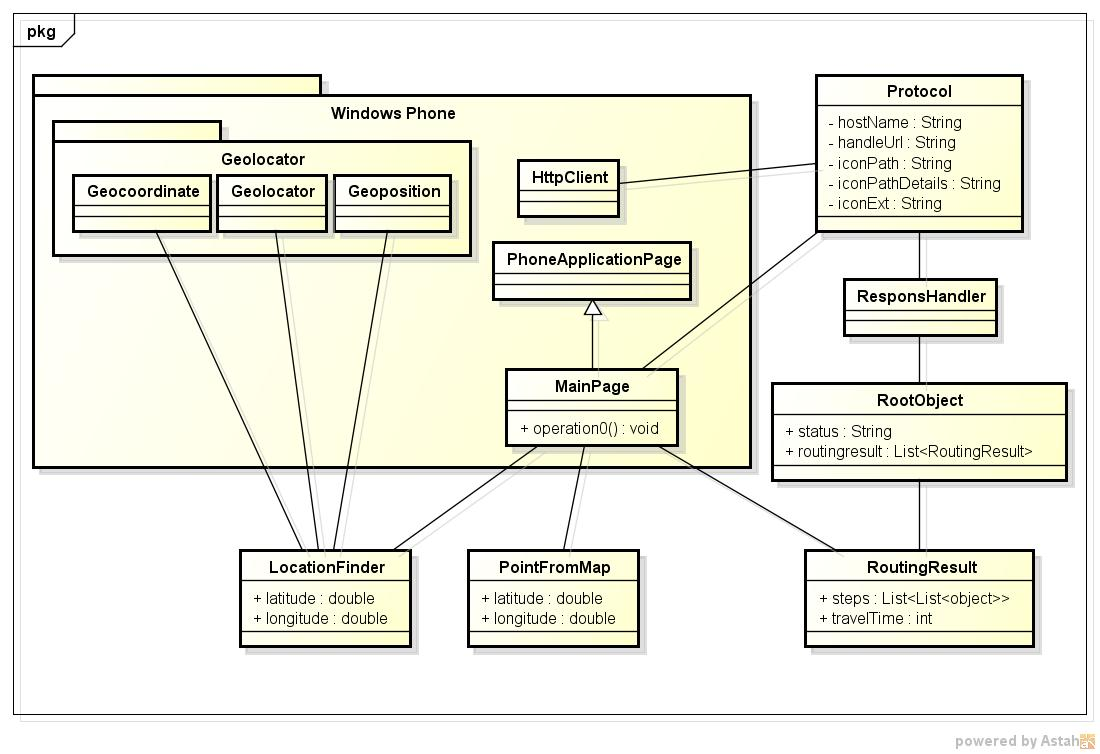
\includegraphics[scale=0.4]{Gambar/useCase_dan_Class/class}
	\caption{Diagram Kelas}
	\label{fig:kelas}
\end{figure}

Berikut deskripsi kelas pada gambar~\ref{fig:kelas}.
\begin{itemize}
	\item Kelas \textit{Protocol} \\
	Merupakan kelas yang menampung semua alamat URL yang berhubungan dengan Kiri API. Semua pemanggilan akan ditangani oleh kelas ini.
	\item Kelas \textit{ResponsHandler} \\
	Merupakan kelas yang menangani masukan dari pemanggilan layanan.
	\item Kelas \textit{RootObject} \\
	Merupakan kelas untuk menampung status dan daftar dari layanan \textit{routing} Kiri API. Hasil kembalian akan dipisahkan di kelas ini untuk selanjutnya ditampung di kelas \textit{RoutingResult}. 
	\item Kelas \textit{RoutingResult} \\
	Merupakan kelas untuk menampung setiap langkah dari rute sesuai masukan pengguna. Pada kelas ini juga rute akan digambarkan pada peta.
	\item Kelas \textit{PointFromMap} \\
	Merupakan kelas yang dapat mengetahui lokasi yang ditunjuk pengguna pada peta. Kelas ini akan menyimpan lokasi yang ditunjuk pengguna dalam bentuk \textit{latitude} dan \textit{longitude}.
	\item Kelas \textit{LocationFinder} \\
	Merupakan kelas yang digunakan untuk mencari lokasi. kelas ini akan memanfaatkan kelas \textit{Geocoordinate} untuk mendapatkan lokasi. Setelah lokasi didapatkan dalam bentuk kelas \textit{Geoposition} maka akan diubah ke \textit{latitude} dan \textit{longitude}. 
\end{itemize}